\chapter{Experimental Results}
\label{chap:results}

This chapter describes the evaluation phase of our defense solution.
Our purpose is to give an estimation of its efficacy and efficiency on different scenarios.
After specifying the configuration of the target system used for our experiments, we define and implement different test cases
and provide the experimental results for each one.


\section{Experiments definition}
\label{sec:exp-def}

To validate our detection system and to estimate its overhead, we performed different experiments.
Given the technical problems described in \mysec{sec:dr-impl} for the Wago PLC version, we chose the Raspberry Pi with CODESYS runtime as target system for our tests.
Note that this system does not have a real-time operating system, and the accuracy of experimental results can be improved by running them on a real PLC.
The system has the same PLC logic and I/O configuration reported in \mysec{sec:attack-pi} for attack analysis.
The attack variants used for tests, instead, are reported in the following sections, because they may differ according to the specific test case.
Finally, the Ghostbuster module has been configured as follows (see \mysec{sec:def-impl} for configuration details):
\begin{itemize}
	\item \itemname{global flags}: \verb|ARCH = arm| and \verb|SOC_MODEL = BCM2835|;
	\item \itemname{I/O monitor}: enabled, active mode, debug disabled;
	\item \itemname{DR monitor}: enabled, active mode, debug disabled;
	\item \itemname{MAP monitor}: enabled, passive mode, debug disabled.
\end{itemize}
For our test cases, we chose $t=10,5,2~\SI{}{ms}$ as most significant monitor scan intervals.

Given the above set-up, in the first phase we evaluate the effectiveness of our solution by estimating the detection rate separately for each monitor.
We discuss about its variation over different values of the monitor scan intervals, both theoretically and with the support of experimental results.
In the second phase, we defined the following test cases to measure the performance overhead:
\begin{itemize}
	\item \itemname{normal conditions}: we measure the overhead during normal PLC logic operations, without any attack or external influence;
	\item \itemname{pin configuration}: we estimate the overhead when a pin configuration attack is executed;
	\item \itemname{pin multiplexing}: same as above, but for a pin multiplexing attack (note that their detection is different, see \mysec{sec:io-design});
	\item \itemname{logic upload}: we provide an estimation of the overhead during the process of uploading a new logic (with a different I/O configuration) to the PLC runtime.
\end{itemize}

To measure the defense overhead, we leveraged Hardware Performance Counters (HPCs).
HPCs allow the user to measure the number of active CPU cycles executed by a system process during a certain amount of time.
The CPU cycles are strictly related to the operations performed by the CPU, since each instruction corresponds to a certain number of CPU cycles.
Basically, the usage scheme of HPCs is made of the following operations:
\begin{enumerate}
	\item reset and start a hardware counter;
	\item wait for target operations to complete, or set a timeout;
	\item read the value contained into the hardware counter.
\end{enumerate}
In ARM processors, hardware counters are managed by a specific component called Performance Monitoring Unit (PMU).
For our purpose, we leveraged PMU by using the following methodology:
\begin{enumerate}
	\item we measure the operations performed by the whole kernel in a definite time interval $t$;
	\item we deploy our detection system (loading the kernel module);
	\item we measure again the whole kernel operations during the same time interval $t$;
	\item we compare the results of the two cases.
\end{enumerate}
To measure the operations performed by the entire kernel, we built a minimal kernel module that uses a PMU hardware counter from kernel space,
thus counting every operation performed in kernel context.
To improve the accuracy of our results, this methodology is repeated several times, separately for each test case defined above.
Moreover, we chose $t$ as multiple of the PLC logic scan cycle, in order to have an estimation of the overhead easily comparable to the PLC timing.
The rest of the chapter reports and describes the results of our experiments.


\section{Detection rate}

This section contains the results of our detection rate analysis for each Ghostbuster monitor.


\subsection{MAP monitor}

Since our MAP monitor implementation does not use any heuristic or statistical approach, it does not introduce any uncertainty window.
In fact, we only have the following two cases:
\begin{itemize}
	\item \itemname{Raspberry Pi}: the MAP monitor is in passive mode, providing just logging information about mapping requests;
		since the PLC runtime uses mapping requests as well, a mechanism to detect malicious requests needs to be implemented (see \mysec{sec:map-impl});
	\item \itemname{Wago PLC}: the MAP monitor is in active mode, denying any possible mapping request from user space; the PLC runtime does not use direct I/O from user space;
\end{itemize}
In the second case, the monitor is able to exactly detect all the attacks from user space. In the first case, instead, a detection rate cannot be defined at all.
Thus, for the rest of this analysis we focus on I/O and DR monitors: both of them execute a time-based protection mechanism.


\subsection{DR monitor}
\label{sec:dr-rate}

Based on our threat model, the attacker may either modify I/O configuration directly or use debug registers to obtain better time accuracy before accessing I/O.
Thus, we can analyse the DR monitor detection rate first, independently from the I/O monitor.
Note that, since the DR monitor disables the user interface, the attacker needs to gain kernel privileges to use debug registers.

Our analysis is based on the fact that the attacker uses debug registers to get a reference time of the PLC logic I/O operations, performed at each scan cycle.
For the following theoretical considerations, we assume a $\SI{10}{ms}$ PLC scan cycle, a DR monitor having a scan interval of $\SI{10}{ms}$ as well,
and a real-time operating system (\ie precise timing operations).
In this configuration, the DR monitor verifies debug registers once per each PLC scan cycle. Since DR monitor and PLC logic are unrelated programs,
they are not synchronised; hence, their reference times are completely independent.
When the attacker modifies a debug register, he gets a debug exception on the exact moment of the next I/O operation.
In the worst case (for the attacker), this will happen $\SI{10}{ms}$ after setting debug registers. When the attacker has gained this timing information,
he can immediately restore the value of the used debug register back to the trusted value. The elapsed time between modification and restoring is our \emph{detection window}.
In this context, our DR monitor already raises the bar for the attacker. In fact, in the original version, the attacker could set debug registers
and keep them as long as he needed (\ie unlimited detection window) in order to intercept all the desired I/O operations.
Since this is no more doable because of our monitor, we consider a more sophisticated version in which the attacker tries to minimise the detection window.

The probability that the attacker gets noticed is equal to the probability that our DR monitor falls within the detection window.
If we make the assumption that both attack and DR monitor are blind and independent, \ie both are uniformly distributed within a scan cycle,
the above probability is the same as the probability that the attacker does not get noticed (\ie the attack comes after the DR monitor check).
Theoretically, with this configuration and hypothesis, we have a $50\%$ detection rate. \myfig{fig:dr-window} shows these two cases.
In the first case the attack is detected because the DR monitor check point occurs within the detection window. Otherwise, it is not detected.
Note that the detection window is the time interval during which the attack can be detected because debug registers are holding a malicious value.
\begin{figure}[h]
\centerline{\includegraphics[width=\textwidth]{res/dr-window}}
\caption{DR monitor detection window \label{fig:dr-window}}
\end{figure}

Intuitively, the closer the DR monitor is to the next I/O operation, the higher is the probability to detect the attack.
Thus, this result can be improved in different ways.
\begin{enumerate}
	\item \label{enum:increase} \itemname{Increase}: the number of checks per scan cycles may be increased, by reducing the monitor scan interval.
		This would increase the probability of detecting the attack.
		For example, consider a monitor interval of $\SI{2}{ms}$, implying that the DR configuration is verified $5$ times per scan cycle.
		In this case, if the attack detection window spans more than $\SI{2}{ms}$ before I/O, the attack would be $100\%$ detected.
		Otherwise, if the attacker is lucky and the window is less than $\SI{2}{ms}$, the detection probability is $50\%$ as before.
		Therefore, considering the whole range of $\SI{10}{ms}$, the total detection rate would increase to $1 \times 0.8 + 0.5 \times 0.2 = 0.9 = 90\%$,
		as confirmed later by our results. This approach, however, may cause too much overhead (see \mysec{sec:overhead}).
	\item \label{enum:randomise} \itemname{Randomise}: the DR monitor could be improved by periodically randomising its reference time; for instance, every $n$ PLC scan cycles,
		it can be programmed to sleep for a random time $t \in [5,15]$ instead of $\SI{10}{ms}$. If $n=1$, the monitor is completely randomised.
	\item \label{enum:synchronise} \itemname{Synchronise}: the monitor can be synchronised with the PLC logic before getting started,
		to verify debug registers as closest to the next I/O operation as possible. The synchronisation can use debug registers as well,
		thus resulting in a precise timing.
\end{enumerate}
Furthermore, the above approaches may be combined to achieve better results.
For instance, combining \ref{enum:randomise} and \ref{enum:synchronise} approaches may be useful to generate minimal time alterations on a synchronised monitor.
In particular, consider a synchronised monitor that is triggered $\SI{1}{ms}$ before each I/O operation.
If we generate a random value $r_i \in [0,1]$ at each cycle $i$, with $r_0 = 1$, we can define a variable monitor interval $t_i = (1 - r_{i-1}) + 9 + r_i = 10 + r_i - r_{i-1}$
instead of fixed $\SI{10}{ms}$. If the PLC I/O operation $i$ is performed at $p_i$ instant, the random interval ensures that the monitor is triggered
in an unpredictable time instant $t \in [p_i-1,p_i]$ (\ie $\SI{0.5}{ms}$ before I/O, on average).
According to the system implementation, the synchronisation may go even closer to the I/O operation.
Since our Raspberry Pi system does not have real-time capabilities, the experiments of such an accurate solution cannot give significant experimental results
(\eg it is even possible that the monitor checkpoint goes \emph{after} the I/O operation).
Therefore, our monitor should first be ported to a real-time system, such as the Wago PLC, to evaluate this approach.

In our previous considerations, we assumed that the attack is blind, hence it can appear at any time within a PLC scan cycle.
Unfortunately, a more sophisticated attack may synchronise itself with the PLC scan cycle by manually watching the target I/O value.
After obtaining a rough synchronisation, it would be able to set a debug register for only a few milliseconds before the next I/O operation,
thus reducing the chances of being noticed. Although we could not properly test it on a real-time environment, the synchronised DR monitor should be able to detect the attack.
The reason is that the attacker can only get an approximate reference time, while the DR monitor is more accurate because it takes advantage from debug registers.
Note that the attacker may also repeat the use of debug register at each I/O operation, but this behaviour dramatically increases the chances of getting noticed.
Moreover, if the attacker wants to get more accuracy, he has to poll the I/O value faster, probably causing a non-negligible performance overhead.
This could be an interesting starting point to include a performance monitor to our detection system, as previously discussed in \mysec{sec:pre-analysis}. 
 
In any case, the results of our analysis and experiments demonstrate that the DR monitor practically raises the bar for the attacker.
We tested the DR monitor with different time intervals (approach \ref{enum:increase}), obtaining the detection rates shown in \myfig{fig:dr-rates}.
\begin{figure}[h!]
\centering
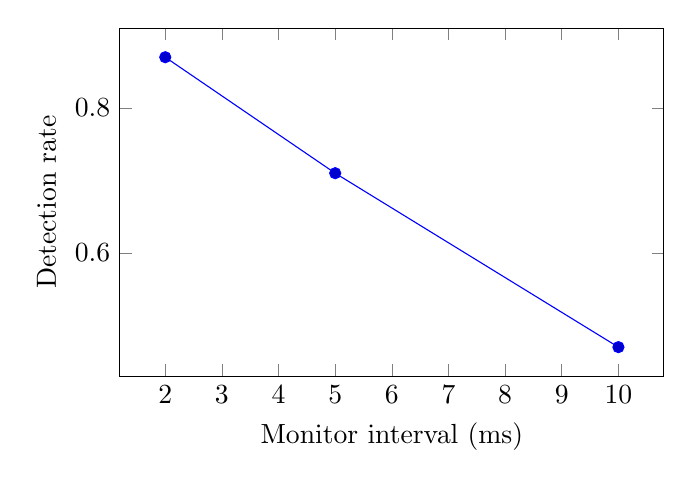
\begin{tikzpicture}
\begin{axis}[xlabel=Monitor interval (ms),xtick={0,1,...,10},ylabel=Detection rate,width=0.7\textwidth,height=6cm]

\addplot coordinates {(2,0.87) (5,0.71) (10,0.47)};

\end{axis}
\end{tikzpicture}
\caption{DR monitor detection rates}
\label{fig:dr-rates}
\end{figure}
The detection rate increases as the monitor scan interval decreases, as expected.
These experimental results confirm our theoretical considerations for approach \ref{enum:increase}, but they are slightly lower then the expected values.
Probably, this is due to the fact that we cannot exactly reproduce uniformly distributed events inside a scan cycle, because the system is not real-time
and the events may depend on the current CPU load. The results are obtained by repeating the following operations $n = 1000$ times:
\begin{itemize}
	\item start the DR monitor;
	\item wait for random time interval (to achieve pseudo-independence);
	\item execute the attack;
	\item wait for enough time to complete a scan cycle;
	\item terminate the attack and stop the monitor;
	\item check whether the attack has been detected or not.
\end{itemize}
The detection rate is computed as $\frac{d}{n}$, where $d$ is the number of detected attacks out of $n$.


\subsection{I/O monitor}

The detection rate analysis for I/O monitor is similar to what we did for DR monitor.
The main difference is that, in order to reach his goal, the attacker will likely need to tamper with many subsequent I/O operations,
while it needs debug registers just once at the beginning.
Thus, the probability of remaining stealth against I/O monitor is the product of all the probabilities of each scan cycle.
For instance, if the probability of being unnoticed within a scan cycle is $0.70$, and the attacker needs at least $20$ operations,
the probability of escaping the detection is $0.70^{20} = 0.0008 = 0.08\%$.
Note that we did not assume a high detection rate for scan cycle ($0.30$), and we only considered $20$ operations, which means just $\SI{10}{ms} \times 20 = \SI{200}{ms}$.

For the I/O monitor analysis, we distinguish the following two cases:
\begin{itemize}
	\item the attacker directly modifies I/O configuration without using debug registers;
	\item the attacker is able to circumvent DR monitor and use debug registers, and modifies I/O configuration in proximity of the PLC I/O operation.
\end{itemize}
In the first case, we do not repeat our considerations because they are similar to what discussed for DR monitor.
For the second case, the attacker can leverage debug registers either for initial synchronisation only, or for each scan cycle.
As discussed in \mysec{sec:dr-rate}, the former case allows the attacker to get an initial starting reference time,
while the latter case is practically unfeasible due to the presence of the DR monitor.
Thus, we assume that the attacker is no more able to be extremely accurate, but it can only change the I/O configuration in proximity of each PLC I/O operation.
In this scenario, if a PLC I/O is performed at time $p_i$, the best approach for the monitor is to check I/O configuration randomly within $[p_i-\epsilon,p_i+\epsilon]$.
Note that this behaviour must be achieved without using debug registers for each scan cycle, because it would cause too much overhead.
Therefore, it must be done manually. However, since in our non-real-time target system we were not able to accurately measure its detection rate, we relaxed the above constraint.
Given a fixed monitor interval $t$ and a random value $r_i$ for each scan cycle, we check I/O configuration every $t_r ~\SI{}{ms}$, with $t_r \in [t-r_i,t+r_i]$.
Thus, $t$ becomes the \emph{average} I/O monitor interval. We tested this monitor against an attack which changes I/O configuration $\SI{0.5}{ms}$ before PLC I/O
and restores it $\SI{0.5}{ms}$ after the I/O operation. We estimate the probability that the attack is detected at each scan cycle, as we did for DR monitor.

The results of our approach are shown in \myfig{fig:io-rates}.
The detection rate $r$ related to one single scan cycle is lower with respect to the DR monitor case, because we used a more sophisticated attack.
However, since the attacker has to repeat the I/O attack for more than one scan cycle to obtain significant effects on the physical process,
we consider the probability of getting noticed after $n$ manipulated scan cycles, which is $1 - (1 - r)^{n}$, where $r$ is the detection rate related to each scan cycle.
Therefore, the probability of remaining unnoticed actually decreases exponentially at each scan cycle.
For instance, given the detection rate $r = 0.2$ of the monitor with $t = 5$, the probability that the attacker
gets noticed after just $10$ scan cycles is $1 - (1 - r)^{10} = 0.89 = 89\%$.
Note that, if the attacker is using debug registers, both DR monitor and I/O monitor detection rates must be taken into account,
making the probability of being detected even higher.
\begin{figure}[h]
\centering
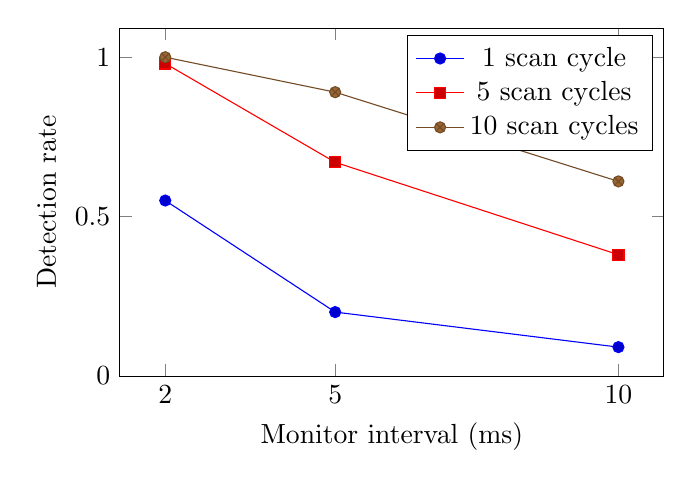
\begin{tikzpicture}
\begin{axis}[xlabel=Monitor interval (ms),xtick={2,5,10},ylabel=Detection rate,width=0.7\textwidth,height=6cm]

\addplot coordinates {(2,0.55) (5,0.20) (10,0.09)};
\addlegendentry{$1$ scan cycle}
\addplot coordinates {(2,0.98) (5,0.67) (10,0.38)};
\addlegendentry{$5$ scan cycles}
\addplot coordinates {(2,0.9997) (5,0.89) (10,0.61)};
\addlegendentry{$10$ scan cycles}

\end{axis}
\end{tikzpicture}
\caption{I/O monitor detection rates}
\label{fig:io-rates}
\end{figure}


\section{Performance overhead}
\label{sec:overhead}

Finally, we evaluate our implementation by measuring the performances in $4$ different test cases, as previously described in \mysec{sec:exp-def}.
Since our overhead is always lower than $1\%$ and our target system is not accurate enough (not real-time),
we could not get reliable results separately for each monitor. Therefore, we provide the overhead estimation for our whole implementation as a function of the monitor time intervals.
We chose $t \in \{2,5,10\}$ as representative time intervals (in $\SI{}{ms}$), which are the same used for detection rate estimation.
In this case, a configuration having time interval $t$ means that both DR and I/O monitor are configured to be triggered every $t~\SI{}{ms}$,
while the MAP monitor remains unmodified among different configurations. The following sections report the results related to the corresponding test case.

\subsection{Normal conditions}

For this test case, we just observed the CPU cycles of the entire system and its PLC runtime, with and without Ghostbuster.
No attacks are executed during the test, to estimate our defense overhead when the system is working under normal conditions,
which on a real PLC is true for most of the time.
The experimental results are reported in \myfig{fig:normal-overhead}, showing CPU cycles over time, in $4$ different configurations:
Ghostbuster deployed with $t=2,5,10$, and without Ghostbuster. The amount of CPU cycles is collected every $\SI{50}{ms}$ ($5$ PLC scan cycles)
by leveraging the specific Performance Monitoring Unit (PMU) counter register.

\begin{figure}[h]
\centering
\begin{tikzpicture}
\begin{axis}[xlabel=Time (s),ylabel=CPU cycles,ymin=9100000,ymax=12200000,width=\textwidth,height=8cm]

\addplot table [y=wg, x=t]{res/normal.dat};
\addlegendentry{Without Ghostbuster}
\addplot table [y=g10, x=t]{res/normal.dat};
\addlegendentry{Ghostbuster $t = \SI{10}{ms}$}
\addplot table [y=g5, x=t]{res/normal.dat};
\addlegendentry{Ghostbuster $t = \SI{5}{ms}$}
\addplot table [y=g2, x=t]{res/normal.dat};
\addlegendentry{Ghostbuster $t = \SI{2}{ms}$}

\end{axis}
\end{tikzpicture}
\caption{Ghostbuster overhead during normal condition}
\label{fig:normal-overhead}
\end{figure}

We estimated the Ghostbuster overhead from the data shown in the plot, considering the average of CPU cycles over time.
When our defense is not present, the system performs $0.992 \times 10^{7}$ CPU cycles on average.
After deploying Ghostbuster, the system consumes $1.019 \times 10^{7}$, $1.049 \times 10^{7}$, and $1.107 \times 10^{7}$ CPU cycles on average,
causing an overhead of $2.72\%$, $5.82\%$, and $11.59\%$ for $t = 10,5,2~\SI{}{ms}$ respectively.
Thus, depending on the target system, the user must choose the best trade-off between detection rate and overhead.
For instance, the solution having a monitor scan interval $t = \SI{2}{ms}$ has a desirable detection rate, but its overhead may be unacceptable for many embedded systems
with limited resources and strict timing requirements.


\subsection{Pin configuration detection}

For this test case (and the following ones), we focused on just one Ghostbuster configuration, having $t = \SI{10}{ms}$.
In fact, the overhead in case of an attack detection is independent from the value of $t$.
The test is conducted in the same way as the previous case, except that in the middle of measurements we execute a pin configuration attack.
\begin{figure}[h]
\centering
\begin{tikzpicture}
\begin{axis}[xlabel=Time (s),ylabel=CPU cycles,width=\textwidth,height=7cm]

\addplot table [y=wg, x=t]{res/pinconf.dat};
\addlegendentry{Without Ghostbuster}
\addplot table [y=g10, x=t]{res/pinconf.dat};
\addlegendentry{Ghostbuster $t = \SI{10}{ms}$}

\end{axis}
\end{tikzpicture}
\caption{Ghostbuster overhead during normal condition}
\label{fig:pinconf-overhead}
\end{figure}
Note that our solution, in order to distinguish a malicious manipulation from a PLC runtime configuration update, sets a watchpoint and looks into the actual PLC logic.
The results are shown in \myfig{fig:pinconf-overhead}.
The plot shows just an instance of our test case. To estimate the detection overhead, we repeated the same test several times.
The overhead has been computed as the extra \emph{detection area} below the red plot line (with Ghostbuster) with respect to the area of the blue graph (without Ghostbuster).
Note that the overhead of the blue plot is entirely related to the attack itself, and it has been excluded from our defense overhead.
Therefore, the estimated overhead of the detection phase for pin configuration attack is $28.75\%$ on average.


\subsection{Pin multiplexing detection}

We reproduced the same test for pin multiplexing attack, whose detection is easier because it does not require debug registers.
The results are shown in \myfig{fig:pinmux-overhead}.
\begin{figure}[h]
\centering
\begin{tikzpicture}
\begin{axis}[xlabel=Time (s),ylabel=CPU cycles,width=\textwidth,height=7cm]

\addplot table [y=wg, x=t]{res/pinmux.dat};
\addlegendentry{Without Ghostbuster}
\addplot table [y=g10, x=t]{res/pinmux.dat};
\addlegendentry{Ghostbuster $t = \SI{10}{ms}$}

\end{axis}
\end{tikzpicture}
\caption{Ghostbuster overhead during normal condition}
\label{fig:pinmux-overhead}
\end{figure}
As for the above test case, the graph reports the results of a particular test instance. 
To estimate the overhead with more accuracy, we repeated the test several times to obtain an average value.
Using the same concept of the extra detection area below the plot line, we found that the overhead is around $5.76\%$ on average.
As expected, it is much lower than the overhead related to pin configuration detection.
Note that, in both cases (pin configuration and pin multiplexing) our monitor is configured as \emph{active}.
Thus, besides the detection, both overheads include the monitor reaction.
In fact, the attack is immediately reverted back after detection, erasing any malicious effect on the PLC output.


\subsection{PLC configuration update}

Our solution is able to automatically recognise malicious I/O configuration, to simplify the job for the industrial operator who wants to upload a new valid configuration to the PLC
without getting a detection alert. We briefly analyse the behaviour of this test case and report our experimental results.
In particular, we re-use the first test case (normal condition, without attack), repeated with and without our defense.
Additionally, while the test is running, we manually upload a new I/O configuration from the PLC CODESYS environment.
Since we assumed that no pin multiplexing is allowed during run-time, we modify pin configuration just by changing a pin from output to input.
To have smaller delays and simplify the tests, we slightly modified the PLC logic, to toggle the output every $\SI{1}{s}$ instead of $\SI{2}{s}$,
and we changed the Ghostbuster wait time according to it. This wait time is the time between a detection of an I/O configuration change, and the decision of accepting or rejecting it.
On Raspberry Pi system, since the output is written only when it is modified, Ghostbuster needs to wait at least $\SI{1}{s}$ as well.
As a safety measure, we let it wait for $\SI{1.2}{s}$. This behaviour is not needed on real PLCs, whose default behaviour is to write at every scan cycle
(\ie waiting for few milliseconds would be enough).

The results of this test case are shown in \myfig{fig:upload-overhead}.
\begin{figure}[t!]
\centering
\begin{tikzpicture}
\begin{axis}[xlabel=Time (s),ylabel=CPU cycles,ymax=30000000,width=\textwidth,height=7cm]

\addplot table [y=wg, x=t]{res/upload.dat};
\addlegendentry{Without Ghostbuster}
\addplot table [y=g10, x=t]{res/upload.dat};
\addlegendentry{Ghostbuster $t = \SI{10}{ms}$}

\addplot[mark=none] coordinates {(0.35,14860549)} node[pin={[align=center]90:{I/O configuration\\modified\\(set watchpoint)}}]{};
\addplot[mark=none] coordinates {(1.35,21817336)} node[pin={[align=center]90:{Check PLC logic\\(watchpoint triggered)}}]{};
\addplot[mark=none] coordinates {(1.55,14415844)} node[pin={[align=center]85:{Configuration\\accepted\\(remove watchpoint)}}]{};

\end{axis}
\end{tikzpicture}
\caption{Ghostbuster overhead during PLC configuration update}
\label{fig:upload-overhead}
\end{figure}
Since the system is highly noisy during this test, because of the active operations on the PLC software, we are not able to estimate the overhead.
However, the experimental result is still interesting to show the operations performed by Ghostbuster.
Since the upload of a new configuration is done manually, we aligned the graphs on the I/O configuration update instant. The update is
performed by the PLC runtime at $t=\SI{0.35}{s}$. At this time, Ghostbuster notices the change and sets the watchpoint to check PLC logic as soon as possible.
The mechanism is asynchronous and the PLC logic is started independently, we do not cause any direct delay on the PLC software.
From now on, Ghostbuster waits for the next interesting I/O operation related to the re-configured pin.
At $t=\SI{1.35}{s}$, when the watchpoint is triggered, Ghostbuster checks if the actual logic operation is conforming with the new configuration detected at $t=\SI{0.35}{s}$.
In this case, the write watchpoint does not refer to our new input pin. Thus, everything is correct and no alert is thrown.
After the timeout $\SI{1.2}{s}$, the trusted configuration is updated inside our module as well, at $t=\SI{1.55}{s}$.
The main overhead in this test case is caused by the watchpoint, but it cannot be accurately estimated because of the excessive noise.
However, since Ghostbuster performs the same operations as for pin configuration attack test case, the overhead should be similar to that test case.
